\chapter{PCB Layout}
\label{ch:pcb-layout}
\begin{figure}[H]
    \centering
    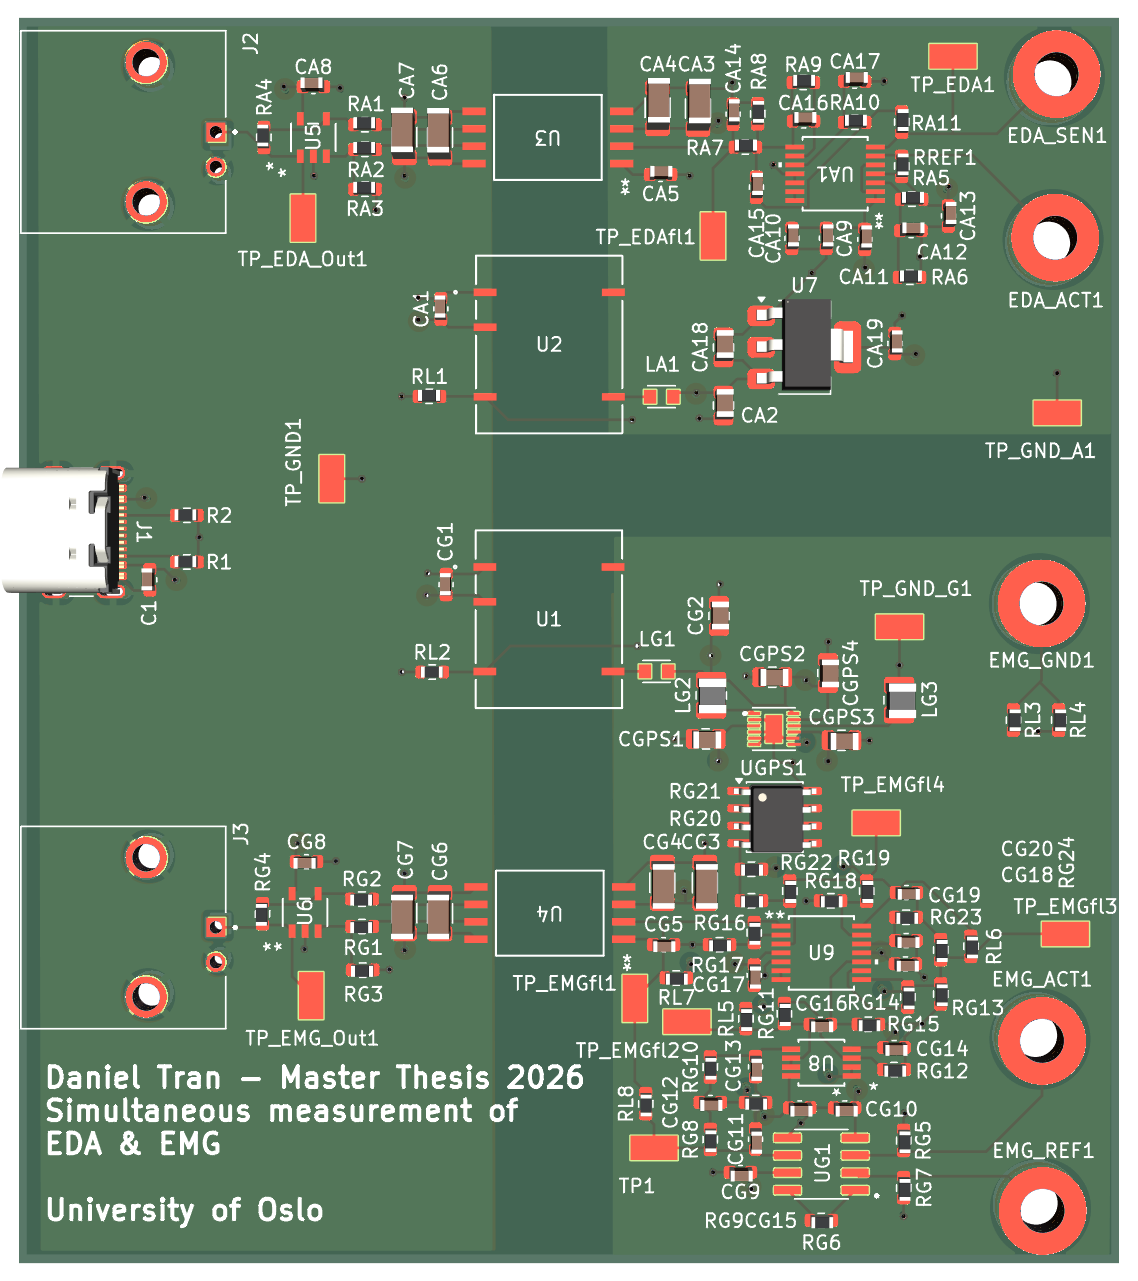
\includegraphics[width=0.8\textwidth, height=0.8\textheight, keepaspectratio]{figures/PCB_layout_version_2.png}
    \caption{Top view of the assembled PCB, KiCad 3D render. Note that component reference designators on the PCB differ from those used in the schematics in Chapter~\ref{ch:methods}: the schematic labels were renumbered for readability in the thesis text, while the PCB silkscreen retains the original KiCad designators from the layout files.}
    \label{fig:pcb-top}
\end{figure}